% -----------------------------------------------------------------
% 2. Arquitectura del Proyecto
% -----------------------------------------------------------------
\section{Arquitectura del Proyecto}

\subsection{Introducción}

El proyecto \textbf{MyBookStore} se concibió inicialmente con una arquitectura
monolítica pero evolucionó a un modelo de
microservicios para mejorar la escalabilidad, la resiliencia y la velocidad de
despliegue continuo.  
Para describir formalmente la solución empleamos
el \emph{C4 Model}\footnote{Desarrollado por Simon Brown, C4 permite
visualizar software en cuatro niveles: Contexto, Contenedores, Componentes y
Código.} y un conjunto de diagramas UML que
facilitan la comunicación técnica con todos los
stakeholders.

% ---------------------------------------------------------------
% 2.1 Modelo C4
% ---------------------------------------------------------------
\subsection{Modelo C4}

\subsubsection{Nivel 1 - Contexto}

\begin{figure}[H]
  \centering
  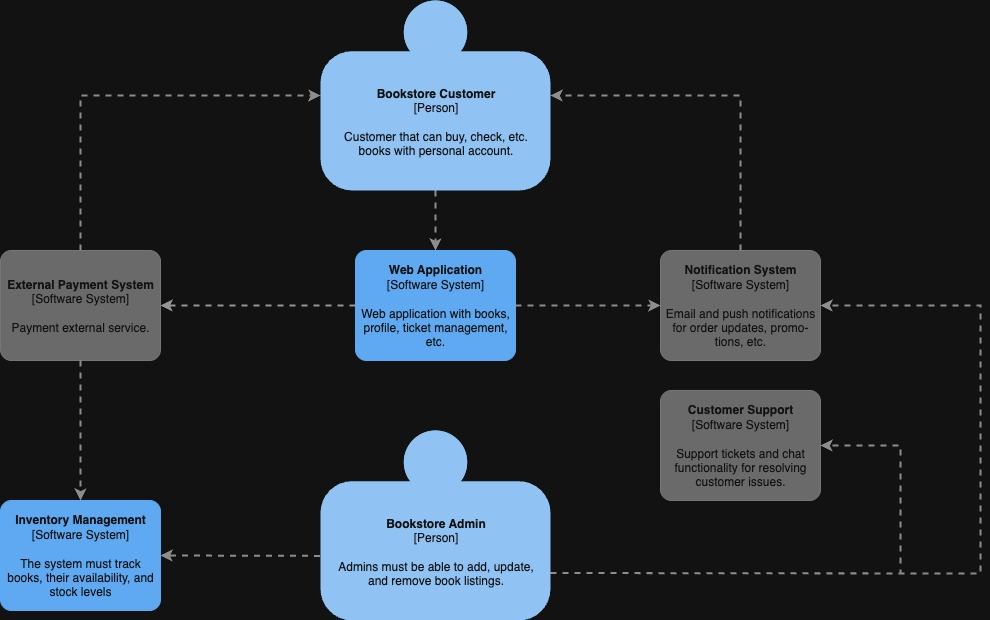
\includegraphics[width=0.9\textwidth]{Figures/2. Architecture/Diagram-C4-Context.jpg}
  \caption{Diagrama C4 - Nivel Contexto.}
  \label{fig:c4-context}
\end{figure}

La figura~\ref{fig:c4-context} muestra a los principales actores (clientes,
administradores y sistemas externos como el \emph{Payment Gateway}) y cómo
interactúan de forma global con \textbf{MyBookStore}.  
Este nivel responde a la pregunta \emph{“¿quién usa el sistema y para
qué?”}.

\subsubsection{Nivel 2 - Contenedores}

\begin{figure}[H]
  \centering
  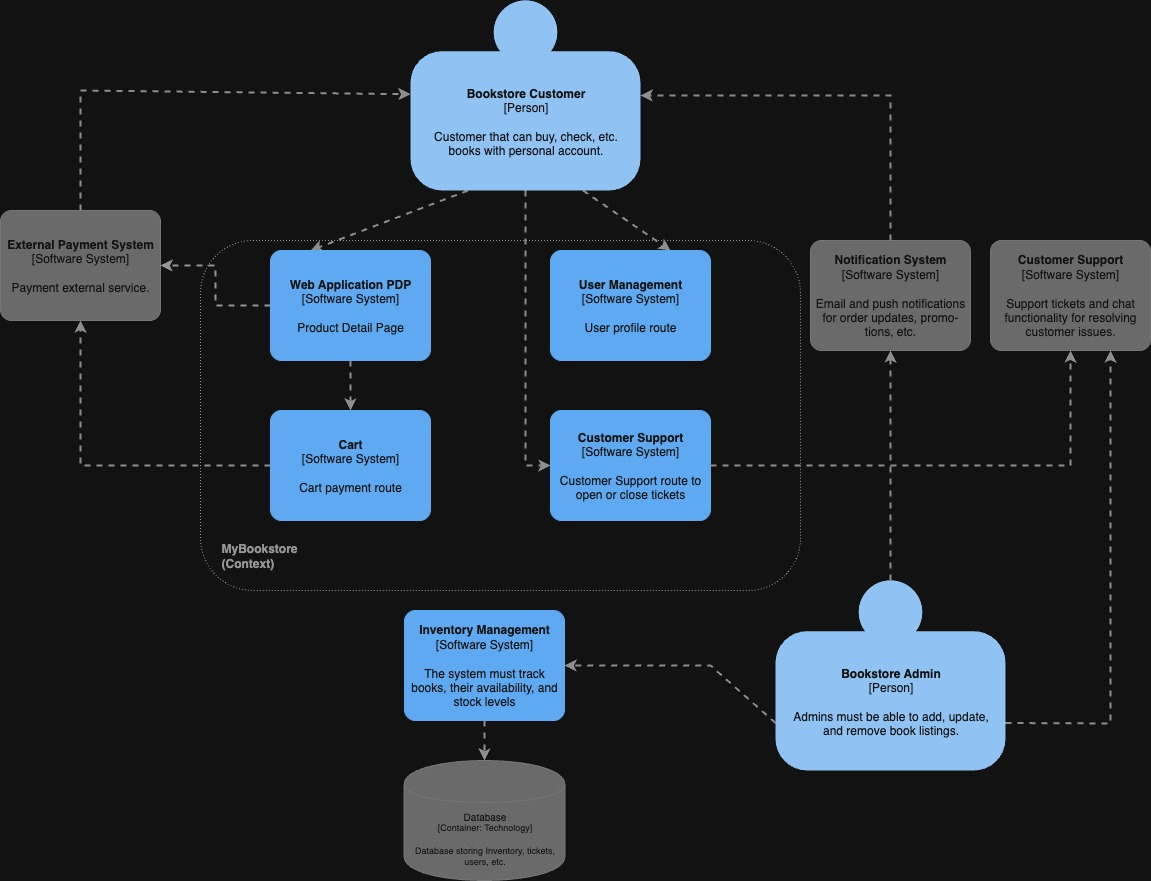
\includegraphics[width=0.9\textwidth]{Figures/2. Architecture/Diagram-C4-Container.jpg}
  \caption{Diagrama C4 - Nivel Contenedores.}
  \label{fig:c4-container}
\end{figure}

El diagrama de la figura~\ref{fig:c4-container} descompone el sistema en
contenedores desplegables (aplicación Web, Carrito, Gestión de Inventario,
Soporte, etc.).  
Cada contenedor encapsula una responsabilidad de negocio clara y expone
interfaces (REST o eventos) que favorecen el bajo acoplamiento.

\subsection{Diagrama de Casos de Uso}

\begin{figure}[H]
  \centering
  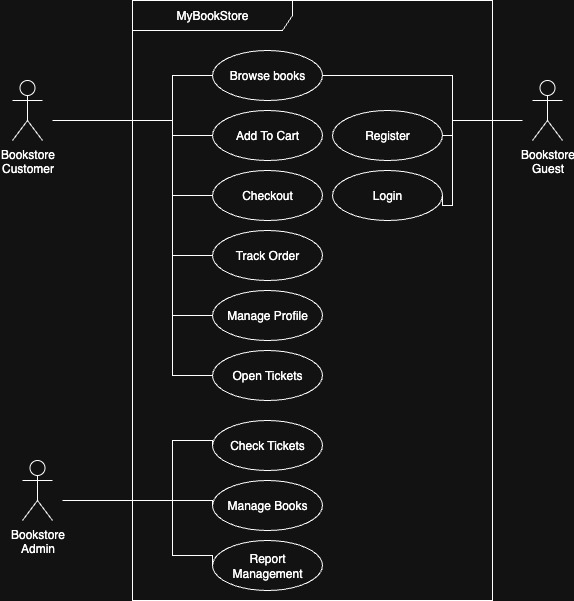
\includegraphics[width=0.55\textwidth]{Figures/2. Architecture/Use-Case-Diagram.jpg}
  \caption{Casos de uso principales de \textbf{MyBookStore}.}
  \label{fig:use-cases}
\end{figure}

El diagrama de la figura~\ref{fig:use-cases} resume las funcionalidades
nucleares que guían el diseño de contenedores y
componentes: desde la navegación y el checkout hasta la
gestión de inventario y la atención al cliente.

% ---------------------------------------------------------------
% 2.2 Vistas de Implementación
% ---------------------------------------------------------------
\subsection{Vistas de Implementación}

\subsubsection{Arquitectura Monolítica Inicial}

\begin{figure}[H]
  \centering
  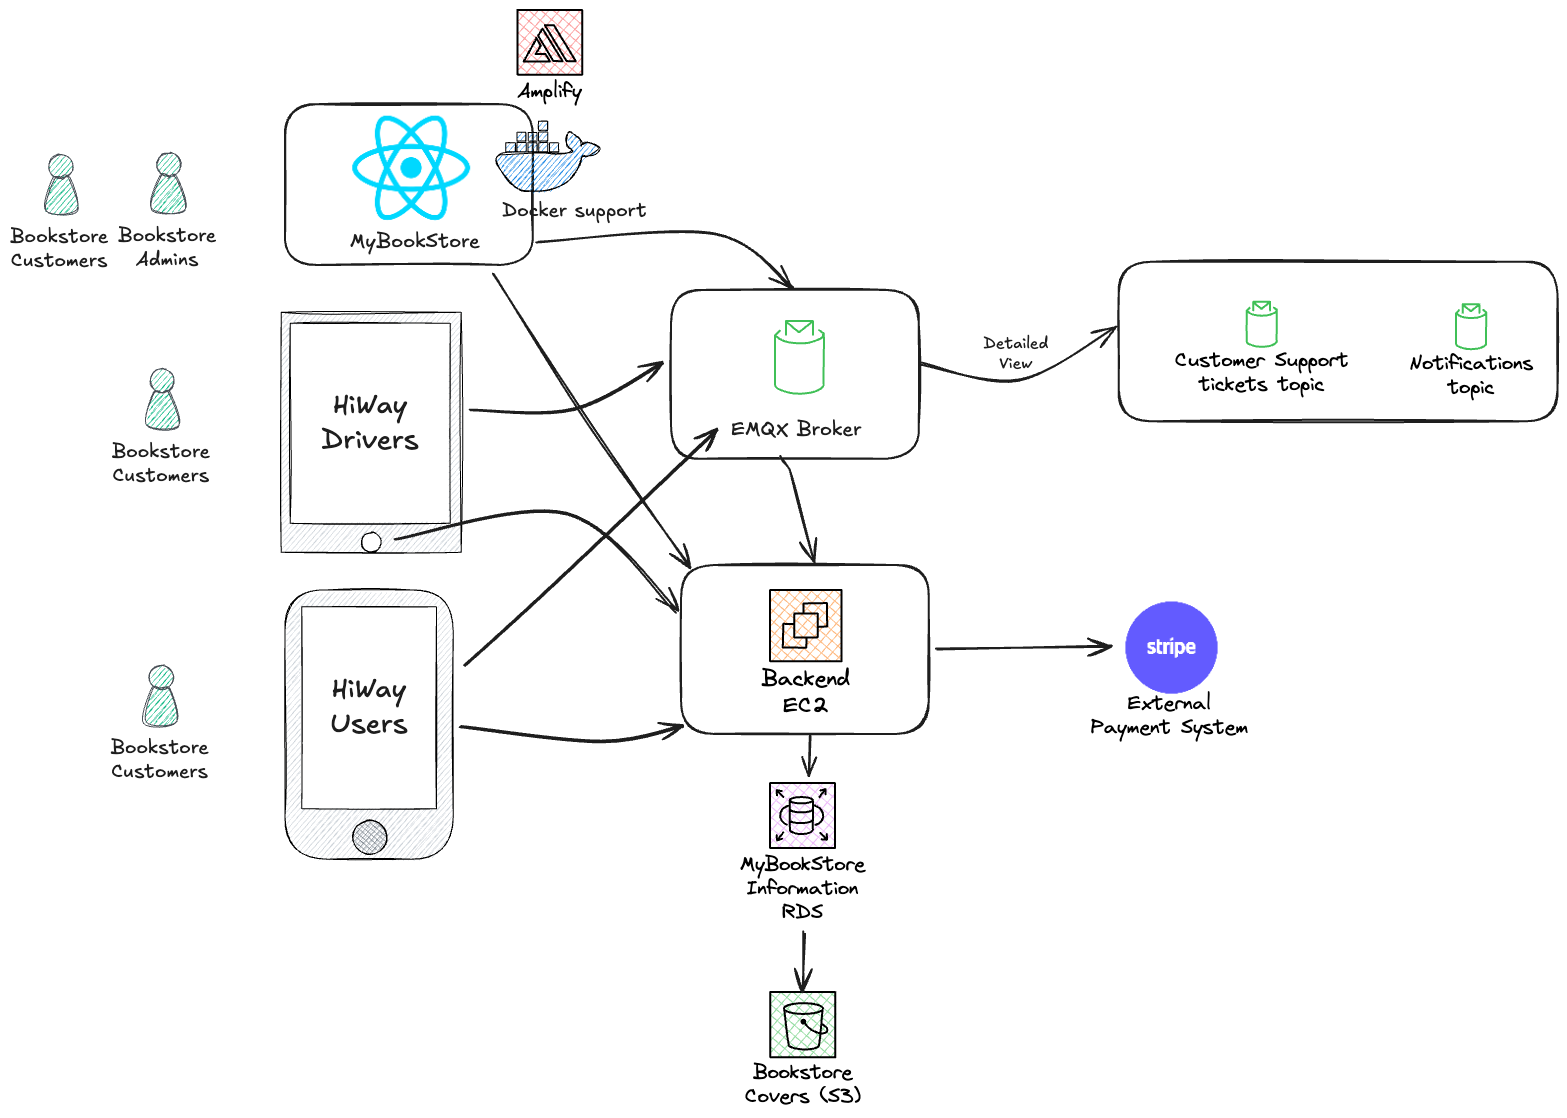
\includegraphics[width=0.9\textwidth]{Figures/2. Architecture/MonolithArchitecture.png}
  \caption{Vista de la arquitectura monolítica desplegada en una instancia EC2.}
  \label{fig:monolith}
\end{figure}

\subsubsection{Arquitectura Basada en Microservicios}

\begin{figure}[H]
  \centering
  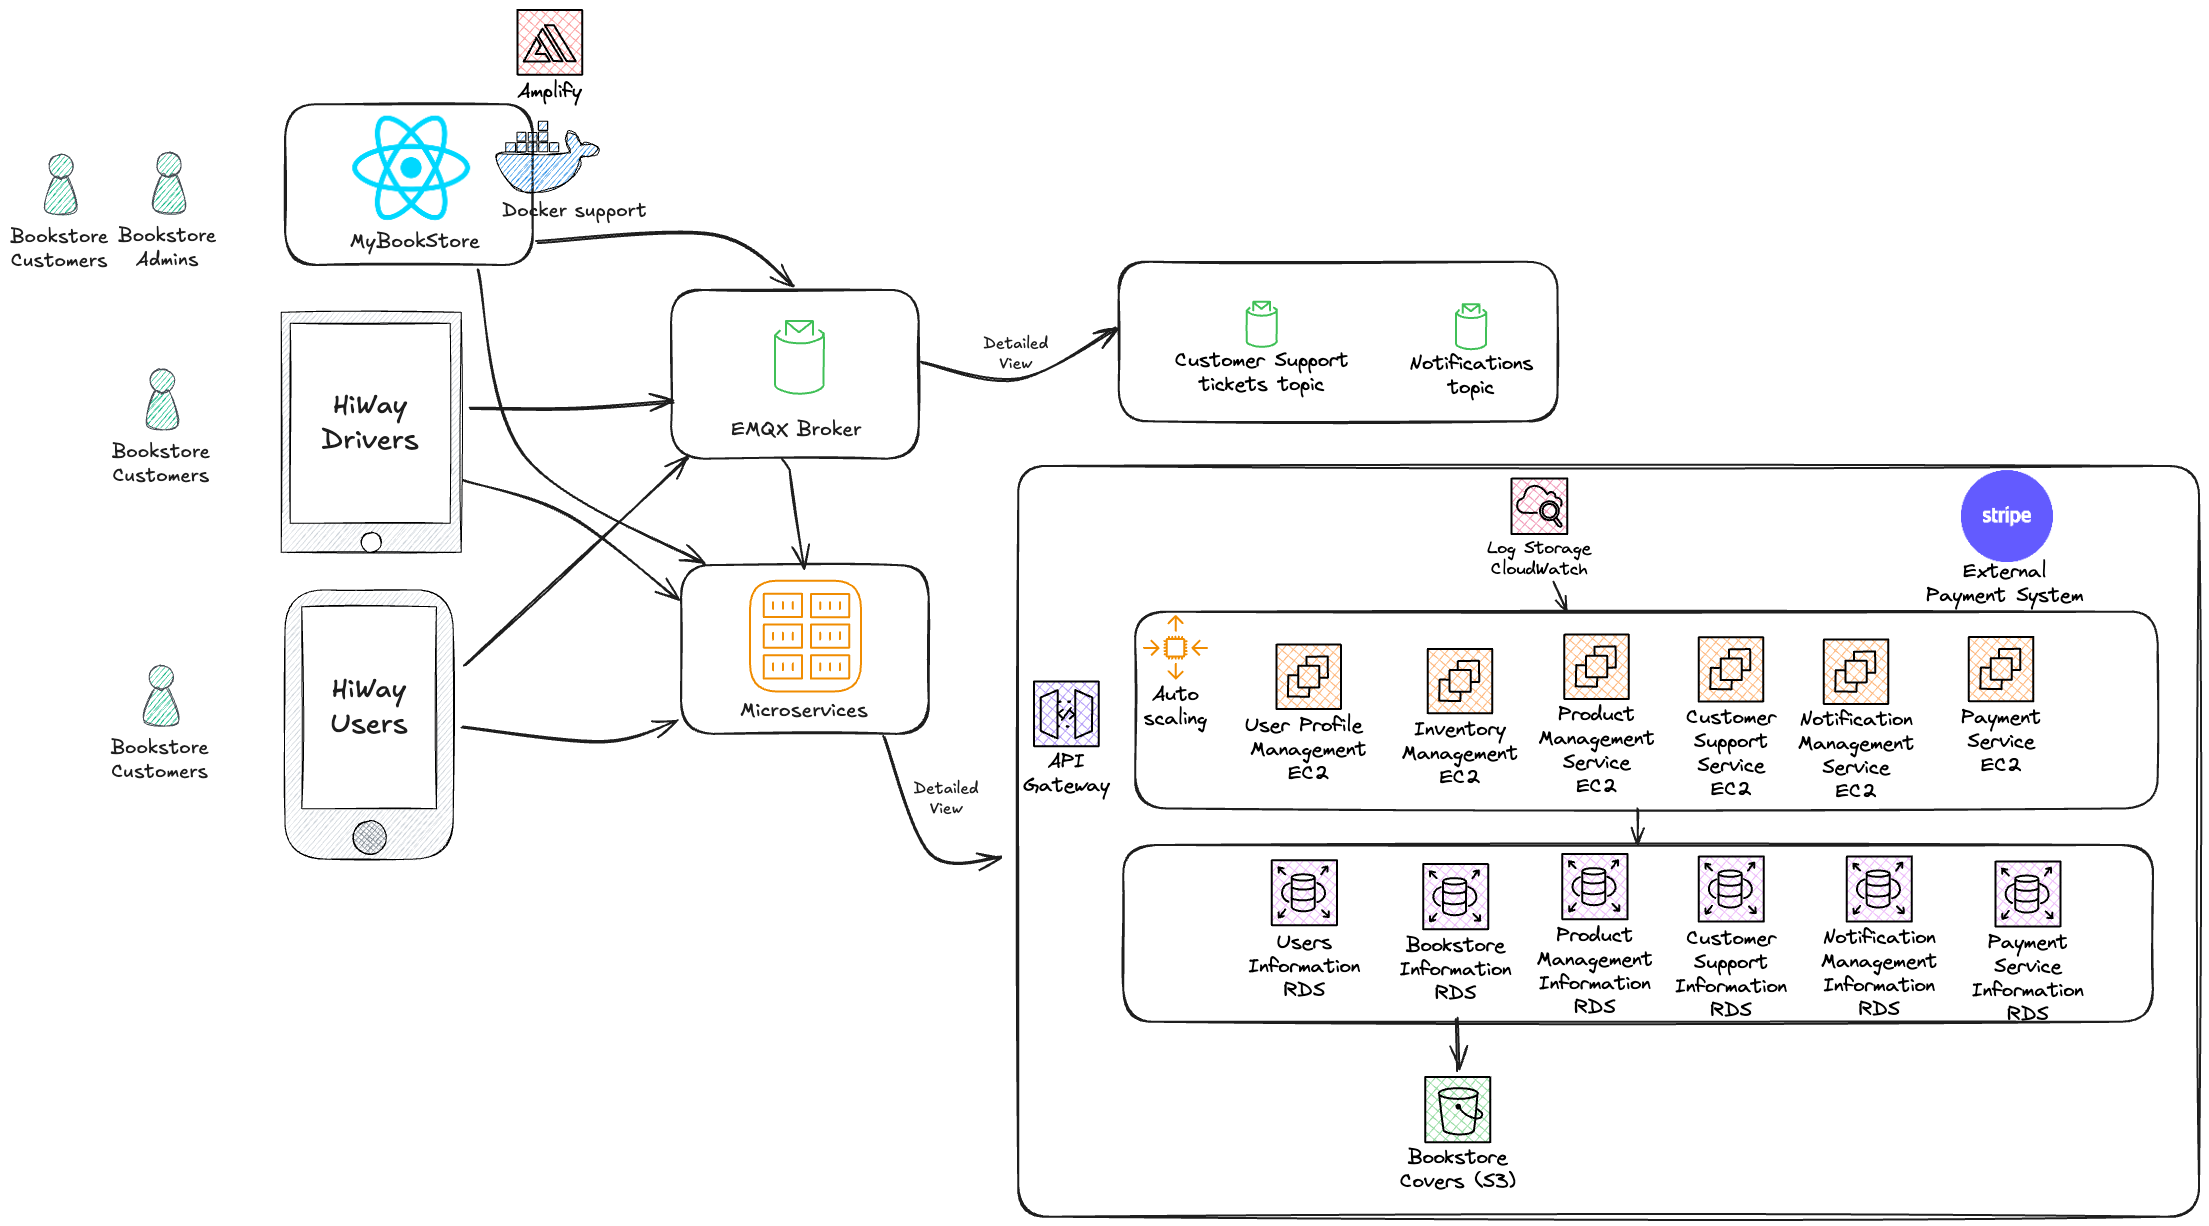
\includegraphics[width=0.9\textwidth]{Figures/2. Architecture/MicroservicesArchitecture.png}
  \caption{Vista de la arquitectura de microservicios con \emph{API Gateway},
           autoescalado y persistencia distribuida.}
  \label{fig:microservices}
\end{figure}

\subsubsection{Comparativa Monolito vs Microservicios}

\begin{table}[H]
\centering
\footnotesize
\begin{tabularx}{\textwidth}{|>{\raggedright\arraybackslash}X|>{\raggedright\arraybackslash}X|>{\raggedright\arraybackslash}X|}
\hline
\textbf{Dimensión} & \textbf{Monolito (Fig.~\ref{fig:monolith})} & \textbf{Microservicios (Fig.~\ref{fig:microservices})} \\ \hline
\textbf{Simplicidad} &
Una base de código y un único artefacto
facilitan el desarrollo inicial y la depuración. &
Mayor complejidad operativa: múltiples
repositorios, canalizaciones de CI/CD y
orquestación (p.\,ej.\, Kubernetes, ECS). \\ \hline
\textbf{Despliegue} &
Cambio atómico: todo el sistema se libera como
un bloque. &
Despliegue independiente por servicio,
permitiendo \emph{canary releases} y rollback
selectivo. \\ \hline
\textbf{Escalabilidad} &
Escalado vertical (más CPU/RAM) o duplicando
el monolito completo. &
Escalado horizontal fino (autoescalado de los
servicios críticos, p.\,ej.\,Inventario o
Checkout). \\ \hline
\textbf{Tiempo de arranque / pruebas} &
Arranque y testeo integrados pero pueden
volverse lentos conforme crece el código. &
Servicios pequeños arrancan rápido; las pruebas
de integración exigen herramientas de
\emph{contract testing}. \\ \hline
\textbf{Evolución del equipo} &
Óptimo para equipos pequeños (\(<\) 5--8
desarrolladores). &
Permite escuadras por dominio de negocio y
libertad tecnológica (polyglot). \\ \hline
\textbf{Resiliencia} &
Fallo de un módulo puede comprometer todo el
sistema. &
Falla aislada al servicio afectado; uso de
\emph{circuit breakers} y reintentos. \\ \hline
\textbf{Costo Operativo} &
Menor al inicio (menos infraestructura y
monitorización). &
Mayor inversión en observabilidad, redes
internas y seguridad de servicio a servicio. \\ \hline
\end{tabularx}
\caption{Ventajas, retos y trade-offs entre monolito y microservicios.}
\label{tab:mono-vs-micro}
\end{table}

\paragraph{Conclusión.}  
El monolito es idóneo para \emph{MVPs} y equipos reducidos; sin embargo,
la demanda prevista de \textbf{MyBookStore} (tráfico variable, picos de
comercio electrónico y necesidad de despliegue continuo) justificó la
transición a microservicios, respaldada por un API Gateway, autoescalado y
observabilidad centralizada.
